\section{XP Virtual Machine and Windbg}
\subsection{Memory leak with Printf}
Nous avons ici deux codes :\\
\begin{center}
\begin{lstlisting}[language=C, caption=Premier programme]
#include <stdio.h>
void main(int argc, char **argv)
{
  printf(argv[1]);
}
\end{lstlisting}
\begin{lstlisting}[language=C, caption=Second programme]
#include <stdio.h>
void main(int argc, char **argv)
{
  printf("%s\n", argv[1]);
}
\end{lstlisting}
\end{center}
\subsection{Understand the difference}
Ces deux codes, une fois compilés, fonctionnent tous les deux de la même manière :
\begin{figure}[H]
  \centering
  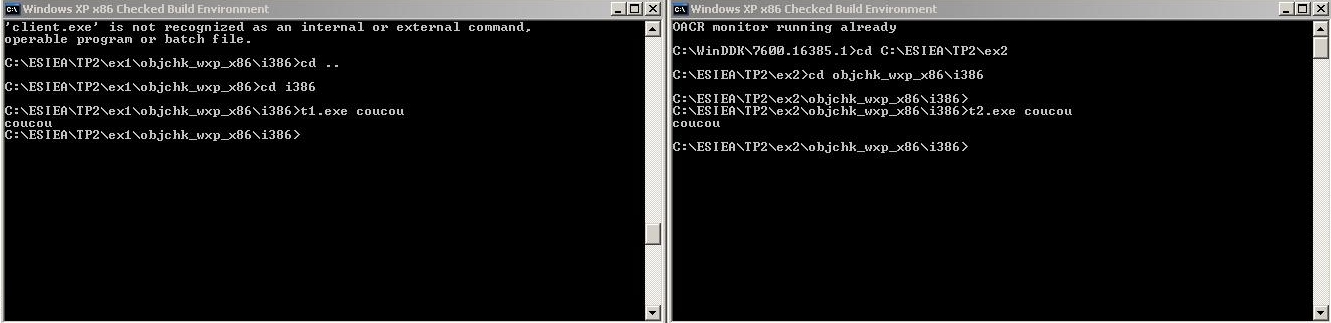
\includegraphics[width=.9\textwidth]{img/200.JPG}
  \caption{Résultat de l'exécution des deux programmes}
  \label{img:1}
\end{figure}

Sur la figure \ref{img:1}, il est possible de voir que ces deux programmes réagissent de la même façon avec l'argument qu'il leur est fournit.
\subsection{Crashing your program}\label{crash}
En exécutant le premier programme avec \enquote{\%s} en paramètre, nous obtenons le résultat suivant :
\begin{figure}[H]
  \centering
  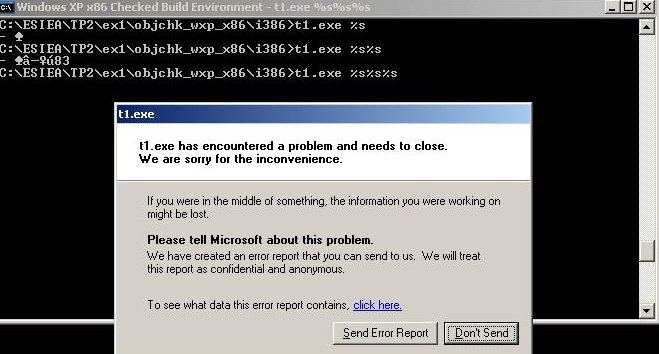
\includegraphics[width=.9\textwidth]{img/201.JPG}
  \caption{Résultat de l'exécution du premier programme avec \enquote{\%s} en paramètre}
  \label{img:2}
\end{figure}
Comme on peut le voir sur la figure \ref{img:2}, il faut trois fois l'argument \enquote{\%s} pour que le programme crash.\\
Le programme va crasher car il va essayer de lire une variable qui n'a jamais été instanciée. De ce fait, lors de l'utilisation de deux \enquote{\%s} dans l'argument, il va accéder à l'espace mémoire dédié au programme. A partir du troisième, il sort de l'espace mémoire alloué et va alors essayer de lire une zone dont l'accès lui est interdit.\\
Cela peut se vérifier en utilisant l'outil \textit{WinDBG}.
\begin{figure}[H]
  \centering
  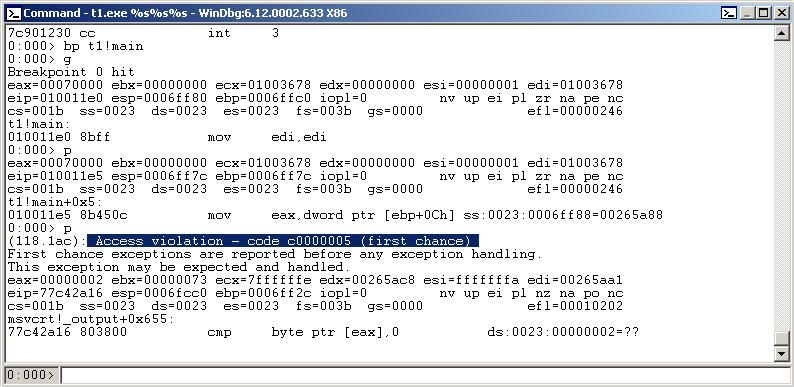
\includegraphics[width=.9\textwidth]{img/202.JPG}
  \caption{Résultat de l'exécution du premier programme avec \textit{WinDBG}}
  \label{img:3}
\end{figure}
Comme on peut le voir sur la figure \ref{img:3}, \textit{WinDBG} nous signale que le programme rencontre une erreur suite à une tentative d'accès sur une zone mémoire non autorisée :
\begin{lstlisting}
(118.1ac): Access violation - code c0000005 (first chance)
First chance exceptions are reported before any exception handling.
This exception may be expected and handled.
\end{lstlisting}
\subsection{Viewing the stack}\label{stack}
Si l'on donne cette fois en argument à notre premier programme la chaîne de caractères \enquote{\%08x}, on obtient le résultat suivant :
\begin{figure}[H]
  \centering
  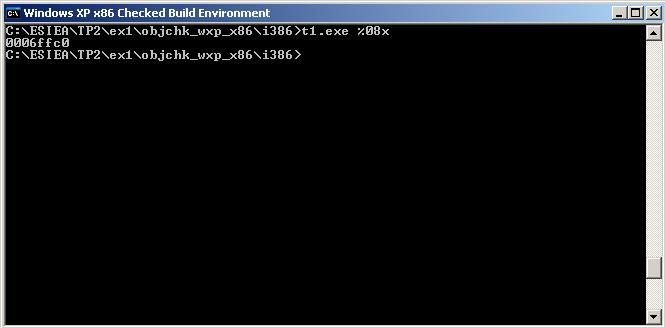
\includegraphics[width=.9\textwidth]{img/203.JPG}
  \caption{Résultat de l'exécution du premier programme avec \enquote{\%08x} en paramètre}
  \label{img:4}
\end{figure}
On se rend alors compte que nous avons ici une adresse mémoire, plus précisément l'adresse $06FFC0$. En effet, cette commande (\enquote{\%x}) va permettre d'afficher une donnée en hexadécimal. Ici, la donnée n'étant pas précisée, elle va donc afficher l'espace mémoire de l'appel.\\
En donnant en argument \enquote{$\%08x\%08x$}, il est possible de retrouver deux valeurs intéressantes du programme. En effet, dans ce dernier il n'y a aucune variable de stockée en mémoire. Ainsi, la première adresse mémoire sur laquelle notre programme va lire avec \enquote{$\%08x$} sera celle d'\textit{EBP}. Cela se vérifie avec l'outil \textit{WinDBG} :
\begin{figure}[H]
  \centering
  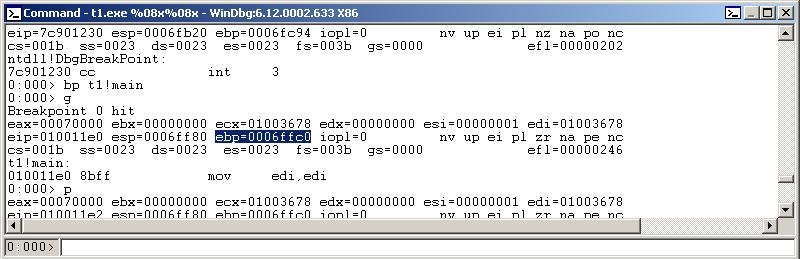
\includegraphics[width=.9\textwidth]{img/206.JPG}
  \caption{État de la mémoire au début de l'exécution du programme}
  \label{img:5}
\end{figure}
Comme on peut le voir sur la figure \ref{img:5}, \textit{EBP} est stocké à l'adresse mémoire $0006FFC0$. Or comme le montre la figure \ref{img:6}, à l'exécution, nous retrouvons cette première adresse sur le prompt du programme.
\begin{figure}[H]
  \centering
  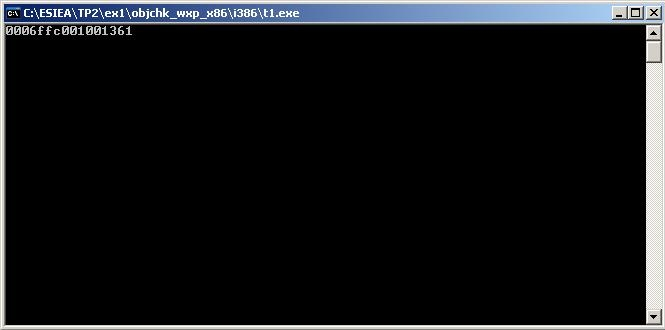
\includegraphics[width=.9\textwidth]{img/205.JPG}
  \caption{Résultat de l'exécution du troisième programme}
  \label{img:6}
\end{figure}
La seconde adresse correspond quand à elle à l'adresse de \textit{EIP}. En effet, nous savons que l'adresse d'\textit{EIP} se situe 4 octets après celle d'\textit{EBP} :
\begin{equation}
  EIP = EBP + 4 = 06FFC0 + 4 = 06FFC4
\end{equation}
\subsection{Overwriting the memory}\label{over}
Nous avons le code numéro trois suivant :
\begin{lstlisting}[language=C, caption=Troisième programme]
#include <stdio.h>
void main(int argc, char **argv){
  int bytes;
  printf("%s%n\n", argv[1], &bytes);
  printf("You input %d characters\n", bytes);
}
\end{lstlisting}
En exécutant ce code avec la chaîne de caractères \textit{coucou}, nous obtenons le résultat suivant :
\begin{figure}[H]
  \centering
  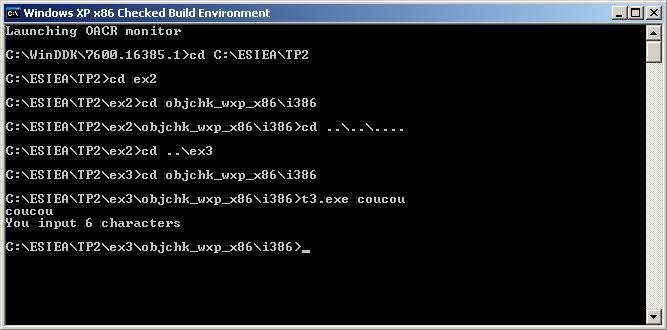
\includegraphics[width=.9\textwidth]{img/204.JPG}
  \caption{Résultat de l'exécution du troisième programme}
  \label{img:7}
\end{figure}
Ici, le programme nous retourne la chaîne donnée en paramètre puis affiche sur une nouvelle ligne :
\begin{quotation}
\textit{ You input 6 characters}
\end{quotation} 
Cette phrase va varier en fonction du nombre caractères donnés en argument. Cela est fait grâce à l'argument \textit{\%n} de la fonction \textit{printf}. En effet, ce dernier va permettre de stocker le nombre de caractères déjà affiché par la fonction \textit{printf}.\\
Ainsi, en exécutant ce programme avec \textit{WinDBG}, il est possible d'observer cela. En effet, en donnant comme argument au programme une chaîne de caractères composée de 24 lettres, nous pouvons observer que le compte est réalisé correctement.
\begin{figure}[H]
  \begin{minipage}{.45\textwidth}
    \begin{figure}[H]
      \centering
      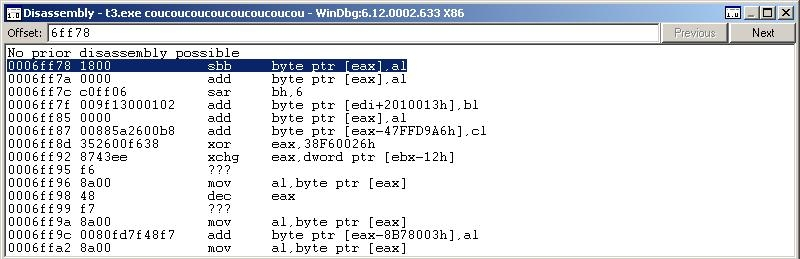
\includegraphics[width=.9\textwidth]{img/207.JPG}
      \caption{Fenêtre \textit{Disassembly} après le premier \textit{printf} du troisième programme}
      \label{img:8}
    \end{figure}
  \end{minipage}
  \begin{minipage}{.45\textwidth}
    \begin{figure}[H]
      \centering
      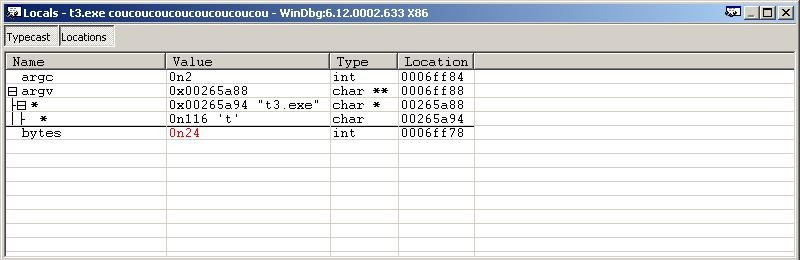
\includegraphics[width=.9\textwidth]{img/208.JPG}
      \caption{Fenêtre \textit{Locals} après le premier \textit{printf} du troisième programme}
      \label{img:9}
    \end{figure}
  \end{minipage}
\end{figure}
Sur la figure \ref{img:8}, nous pouvons lire que l'adresse mémoire $06FF78 (EBP - 4)$ dans laquelle est stockée la variable \textit{bytes} a pour valeur $0x18$\footnote{24 en décimal}. Sur la figure \ref{img:9}, on va aussi pouvoir retrouver la valeur de la variable, cette fois égale à $0n24$.\\
Ainsi, on peut confirmer que la taille de l'argument à bien été comptée.